\appendix
\chapter{Dataset}
\begin{figure}[htb]
  \centering
  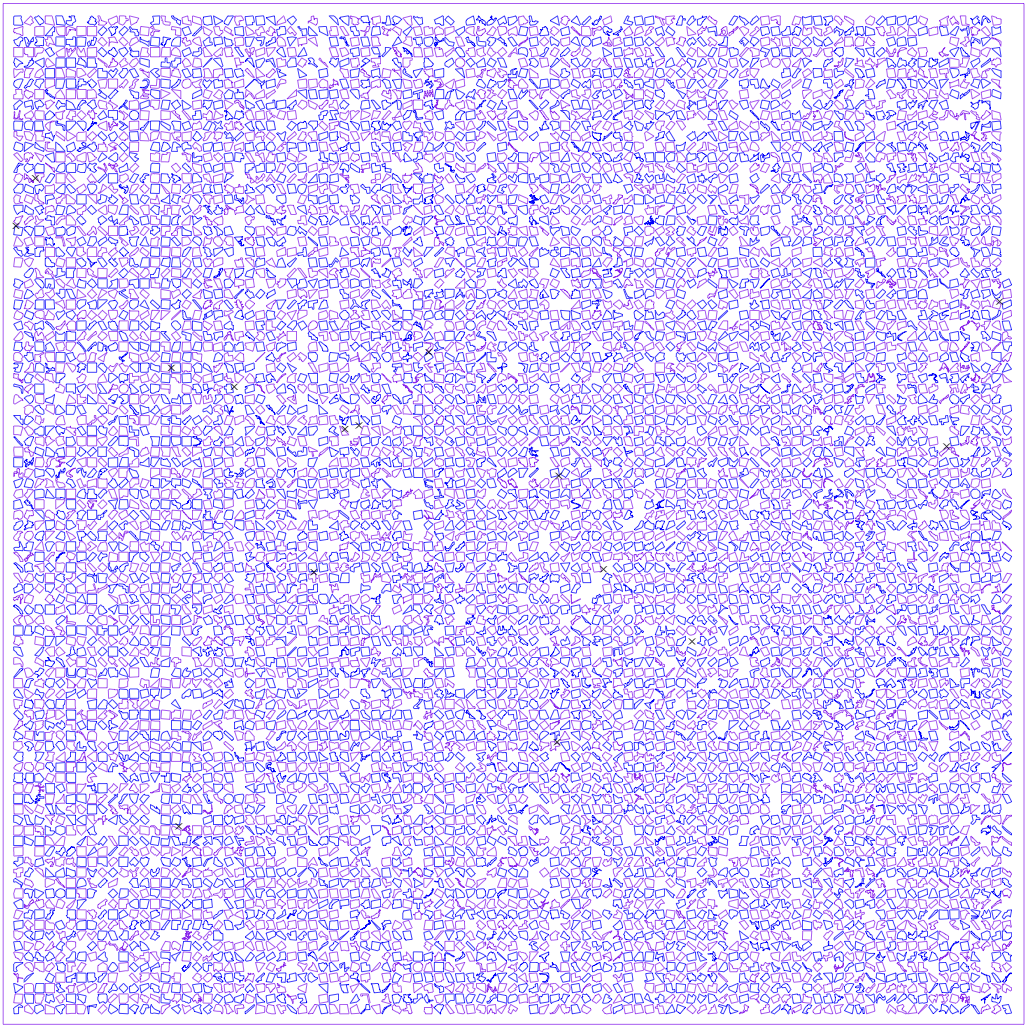
\includegraphics[width=\linewidth]{./pic/poly9000.png}
  \caption{\small The map in experiments, it has nearly 9000 polygonal obstacles, and 10,000
  vertexes.}
\end{figure}
\chapter{Source Code}
\lstinputlisting[caption=extract shape of parks, label=park2poly]{./code/park2poly.h}
\newpage
\lstinputlisting[caption=generate targets, label=gentarget]{./code/genPoints.h}
\newpage
\lstinputlisting[caption=target heuristic, label=heuristic_function]{./code/heuristic}
\newpage
\lstinputlisting[caption=final OkNN, label=oknn]{./code/knnheuristic.cpp}
\newpage
